\section{MOC Pipeline Replica}\label{sec:methodology}
As part of our goal to evaluate the performance of each of the components in the pipeline, the first step was to create a replica of the original pipeline described by \citet{cleggRecalibrationMarsScience2017}
Since we did not have access to the original source code implementing the pipeline, we have replicated it at accurately as we could based on the available information.
We have had to make some assumptions due to insufficient information regarding some components, which we detail in this section.
In addition, some aspects of the pipeline rely on qualitative assessments made by the original authors --- something we cannot do because we are not domain experts.
Consequently, our pipeline is not identical to the original, but we have strived to make it as close as possible while favoring conservative choices and omitting implementations where information about the original pipeline was unclear.
This decision was driven by the aspiration to ensure that the baseline results remained minimally influenced by our methodological choices.

This section is dedicated to describing the methodology of our pipeline, how it differs from the original, and which design choices we have made and why.
Furthermore, we delve into the experiments we have conducted to evaluate the performance of our pipeline such that we can identify the components that contribute the most to the overall error.

Section \ref{sec:methodology_pls1}, we focus on the specifics of the PLS1-SM phase, detailing its associated data preprocessing procedures.
In Section \ref{sec:methodology_ica} then details the ICA phase, including its unique data preprocessing steps.
Lastly, Section \ref{sec:methodology_moc} presents a description of the MOC phase of the pipeline.

\subsection{PLS1-SM}\label{sec:methodology_pls1}
The PLS1-SM phase in our pipeline largely follows the same approach as described in \citet{andersonImprovedAccuracyQuantitative2017} with a few exceptions.
We detail our approach and the differences from the original pipeline in this section.

\subsubsection{Data Preprocessing}\label{sec:pls1_data_preprocessing}
The preprocessing of the data is illustrated in Figure~\ref{fig:pls_data_preprocessing}.

\begin{figure}
	\centering
	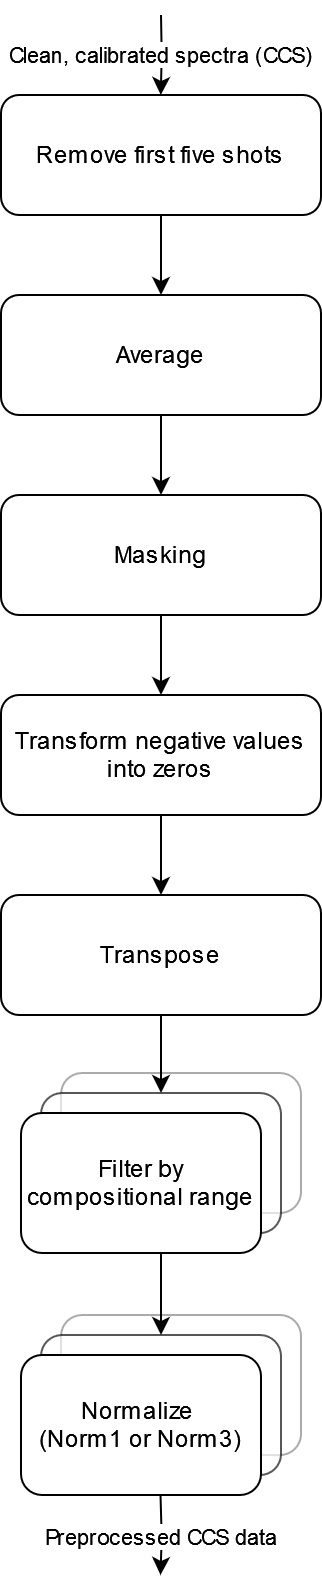
\includegraphics[width=0.175\textwidth]{images/pls_preprocessing.png}
	\caption{The PLS1-SM data preprocessing phase in our recreation of the pipeline. The filtering and normalization steps are done independently for each oxide.}
	\label{fig:pls_data_preprocessing}
\end{figure}
\noindent
We start by removing the first five shots from the data similarly to \citet{cleggRecalibrationMarsScience2017} since they are typically contaminated by dust that covers the target before being removed by the laser-produced shock waves.
Then the remaining 45 shots from each location are averaged, resulting in a single spectrum per location with a total of five spectra per target.
As mentioned in Section~\ref{sec:data_overview}, the edges of the spectral regions contain noise, so we apply masking to the data by zeroing out these regions.
The dataframe is then transformed through a transpose operation, swapping the rows and columns.
This gives us a dataframe with the average intensities per sample as rows, and the wavelengths as columns.
All negative values are then transformed into zeros since negative values are not physically possible.
Given the compositional ranges for each submodel defined in \citet{andersonImprovedAccuracyQuantitative2017}, we filter out the samples whose compositional values are outside of these ranges.
The range is defined by an upper and a lower bound, and any wavelength outside of this range is removed.
Finally, we apply two different normalization techniques, Norm1 and Norm3, to the data.
This results in two separate datasets, each normalized in a distinct manner but derived from the same original dataset.
ICA and PLS-SM are then performed on each of these datasets separately.
The reason for this is that, as \citet{cleggRecalibrationMarsScience2017} found, some of the oxides are better modeled with data normalized using Norm1, while others are better modeled with data normalized using Norm3.

\subsubsection{PLS1-SM Regression}\label{sec:methodology_pls1-sm_regression}
The PLS phase of the pipeline follows a submodel approach to make wt. \% predictions for each oxide, as previously mentioned in Section~\ref{sec:introduction}.

%TODO add information about the hyperparameters used
The training of the models follows the same approach as described in \citet{andersonImprovedAccuracyQuantitative2017} and is illustrated in Figure~\ref{fig:pls_training}.
However, assumptions have been made regarding the k-fold cross-validation process, as the authors are ambiguous in their description of the number of folds used.
We interpreted their description as using a 20\% holdout split and a 4-fold on the remaining 80\% of the data --- resulting in a total of 5 folds.
Furthermore, we have decided to automate outlier removal as described in Section~\ref{sec:methodology_outlier_removal} rather than performing it manually.
Finally, similar hyperparameters have been used for the PLS models as described in \citet{andersonImprovedAccuracyQuantitative2017}.

\begin{figure}
	\centering
	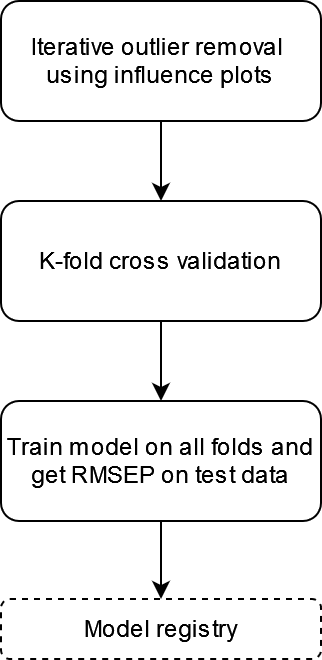
\includegraphics[width=0.175\textwidth]{images/pls_training.png}
	\caption{The PLS1-SM training phase in our recreation of the pipeline. This phase is repeated for each oxide's compositional range.}
	\label{fig:pls_training}
\end{figure}

Obtaining predictions for each of the eight oxides, for a single spectrum, requires a separate predictions for each oxide. While PLS regression is capable of multivariate regression, each oxide calls for different hyperparameter configurations and normalization procedures.
The submodels for an oxide generally include a full model, a low, mid, and high model. They are named after the compositional range in the data they are trained on. Here, compositional range refers to the known compositional values for a sample, which we use to filter the sample data to include samples data within that range.
These compositional ranges overlap, which creates a blending range.
Some oxides have only two compositional ranges, which means the model may have low-high as a blending range.

As mentioned, the PLS submodels approach is repeated for each oxide and is illustrated in Figure~\ref{fig:pls_inference}.
Given some new data sample, the full model gives an initial compositional prediction for its oxide.
Based on this prediction, the data is then "binned" into one of five concentration ranges -- the three submodel ranges and two blending ranges.
For each of these five concentration ranges, there is one or two corresponding \textit{submodel(s)}.
These submodels are used to make predictions in the corresponding concentration range after the full model has made its initial predictions.
The submodels are specialized in either low, mid, or high concentration ranges, which are defined in Table 2 in \citet{andersonImprovedAccuracyQuantitative2017}.
If the full model predicts a concentration that falls within a blending range, the approach described in Section~\ref{sec:pls_submodels} is used to combine the predictions from the corresponding submodels.

\begin{figure}
	\centering
	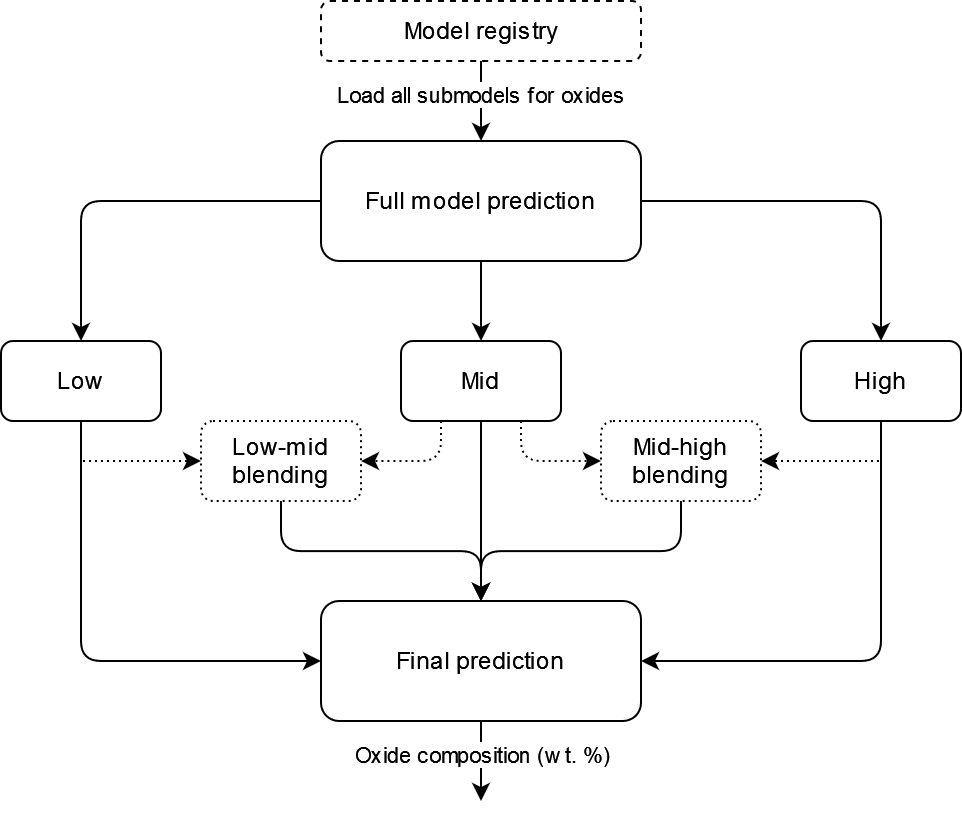
\includegraphics[width=0.45\textwidth]{images/pls_inference.png}
	\caption{The PLS1-SM inference phase in our recreation of the pipeline.}
	\label{fig:pls_inference}
\end{figure}

\subsubsection{Outlier Removal with Mahalanobis Distance and Chi-Squared Test}\label{sec:methodology_outlier_removal}
As mentioned in section \ref{sec:outlier_removal}, if the Mahalanobis distances can be shown to follow a chi-squared distribution, then the chi-squared test can be used to determine whether a sample is an outlier.
Since we do not have the expertise to make a qualitative assessment of the outliers, we have instead decided to use this property of the Mahalanobis distances to automatically detect outliers.
This works by computing the Mahalanobis distance for each data point in the training set, followed by a comparison of these distances against a chi-squared distribution.
A data point is classified as an outlier if its Mahalanobis distance corresponds to a chi-squared statistic that exceeds the critical value of the chi-squared distribution, which is determined by the specified degrees of freedom $\nu$.
The critical value is determined by the significance level $\alpha$ and $\nu$.
Since we have leverage and spectral residuals as our two dimensions, we have $\nu = 2$, because the number of dimensions is equal to the number of degrees of freedom\cite{aggarwal_outlier_2017}.

The outlier removal process is done iteratively because of the phenomenon described in \citet{cleggRecalibrationMarsScience2017} where removing outliers can cause new outliers to appear.
The process is as follows:
\begin{enumerate}
    \item Compute the Mahalanobis distances for each sample in the training set.
    \item Determine chi-squared statistics for these distances.
    \item Eliminate outliers exceeding the chi-squared critical value.
    \item Train a new model on the remaining samples.
    \item Repeat until model no longer improves as measured by the RMSE.
\end{enumerate}

It should be noted that our outlier removal process is conservative to avoid removing too many samples and as such, we have set our significance level $\alpha$ to 0.975.
This means that we are willing to accept a 2.5\% chance of falsely removing a sample that is not an outlier.

Figure~\ref{fig:FeOT_oxide_removal} illustrates running the outlier removal process on the FeOT full model.
As can be seen, the number of outliers decreases with each iteration, and the model improves as measured by the RMSE.
Here, the process terminates after four iterations, as the RMSE no longer improves with further iterations.

\begin{figure*}[]
\centering

% First Row
\begin{subfigure}{.5\textwidth}
    \centering
    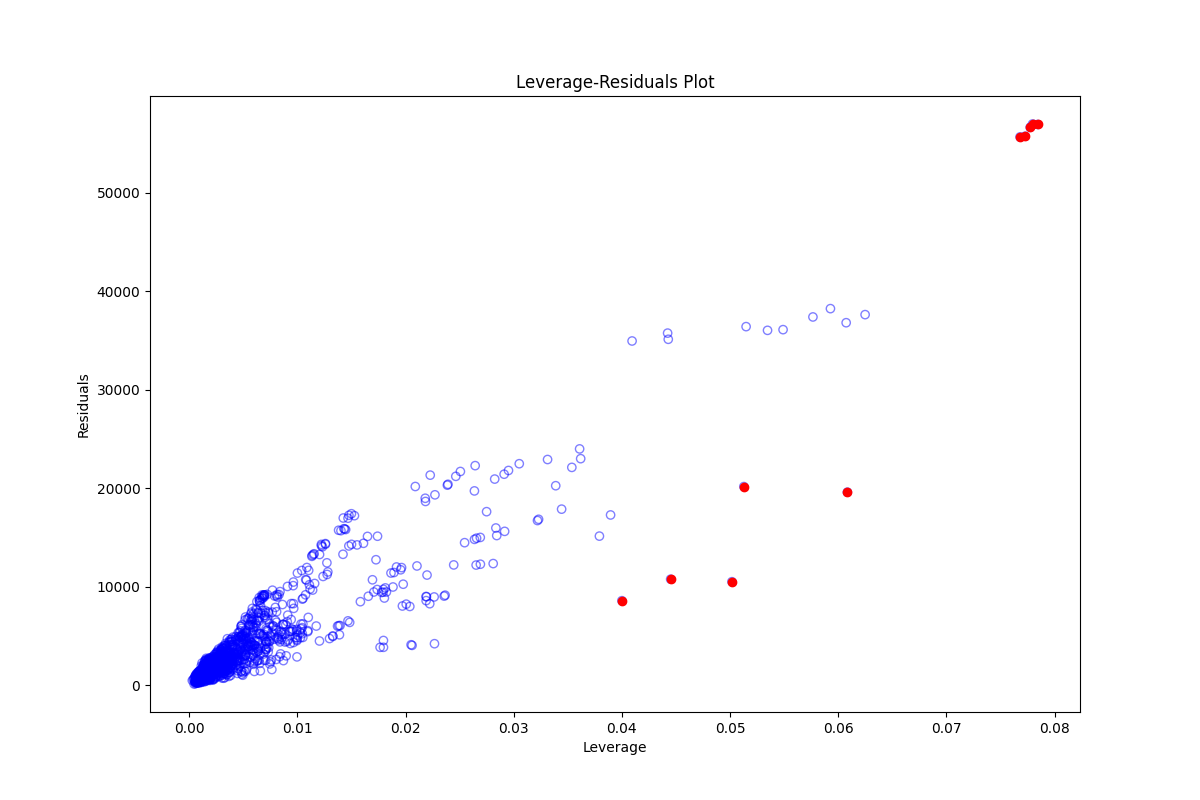
\includegraphics[width=0.9\linewidth]{images/FeOT_Full_1.png}
    \caption{Iteration 1 (RMSE = 2.03)}
    \label{fig:iteration1}
\end{subfigure}%
\begin{subfigure}{.5\textwidth}
    \centering
    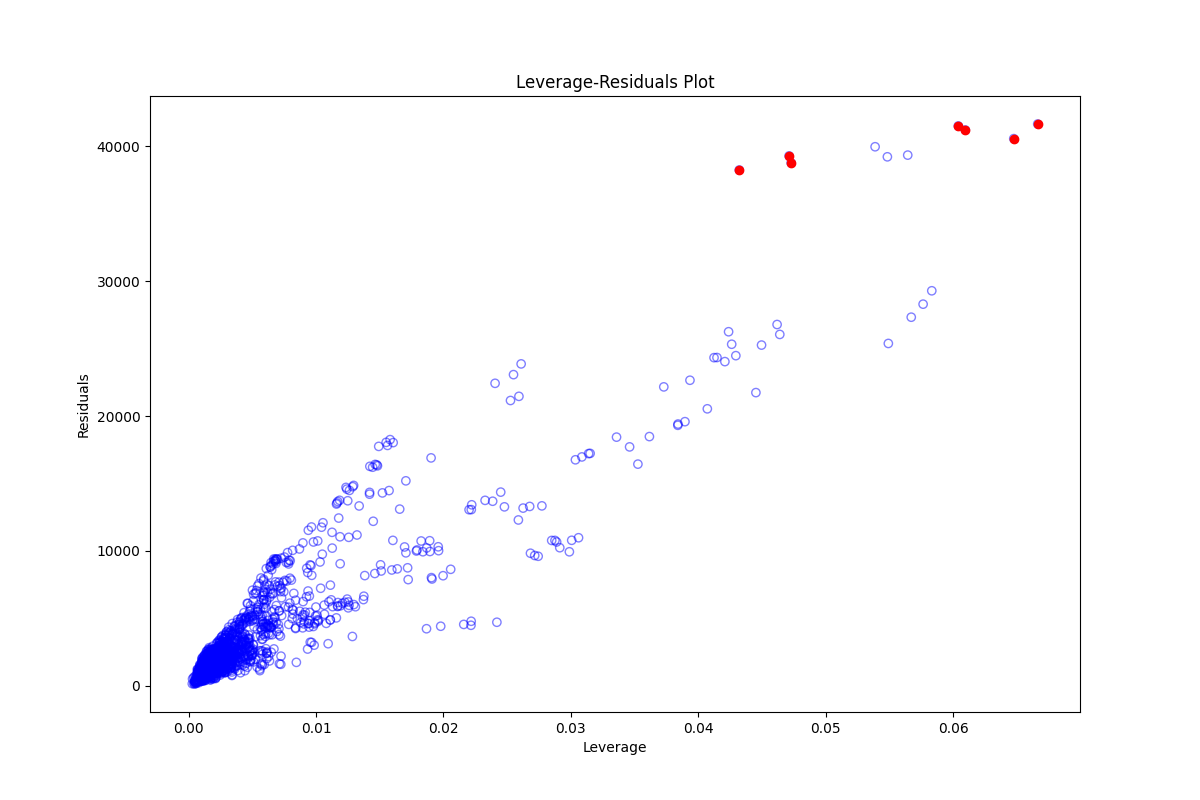
\includegraphics[width=0.9\linewidth]{images/FeOT_Full_2.png}
    \caption{Iteration 2 (RMSE = 1.99)}
    \label{fig:iteration2}
\end{subfigure}

% Second Row
\begin{subfigure}{.5\textwidth}
    \centering
    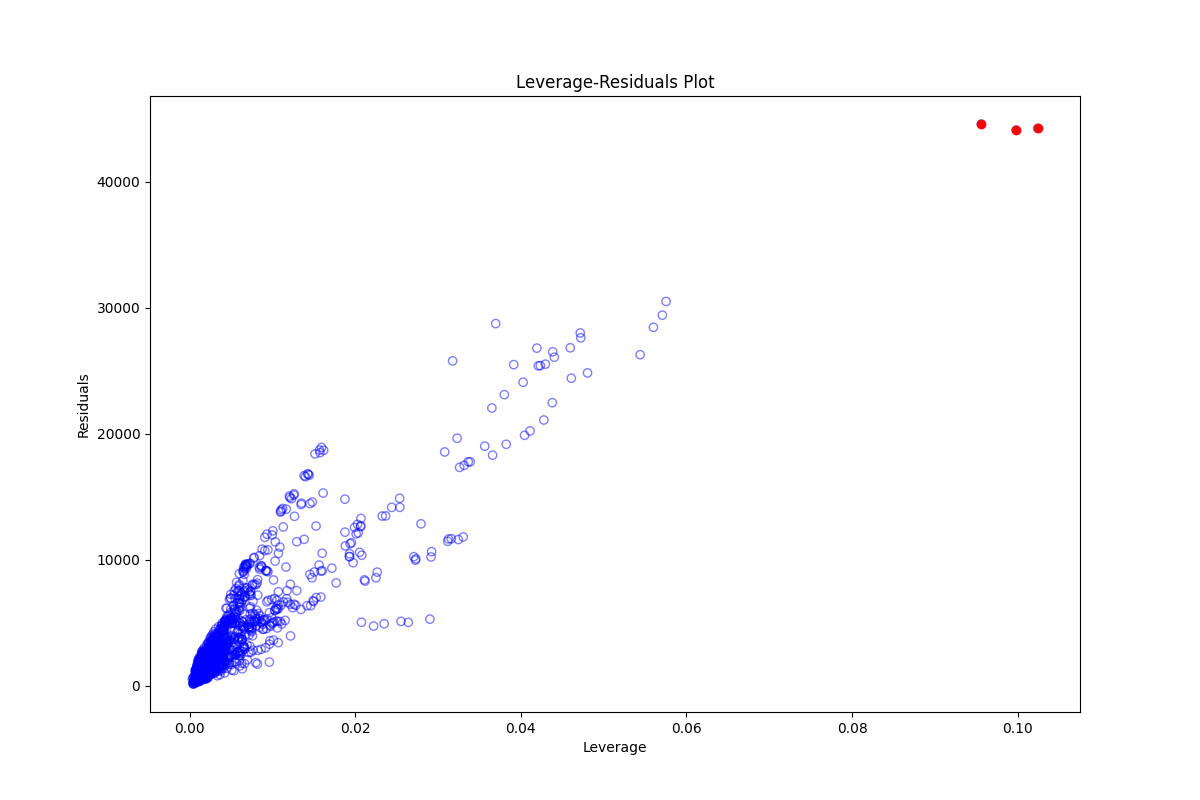
\includegraphics[width=0.9\linewidth]{images/FeOT_Full_3.png}
    \caption{Iteration 3 (RMSE = 1.92)}
    \label{fig:iteration3}
\end{subfigure}%
\begin{subfigure}{.5\textwidth}
    \centering
    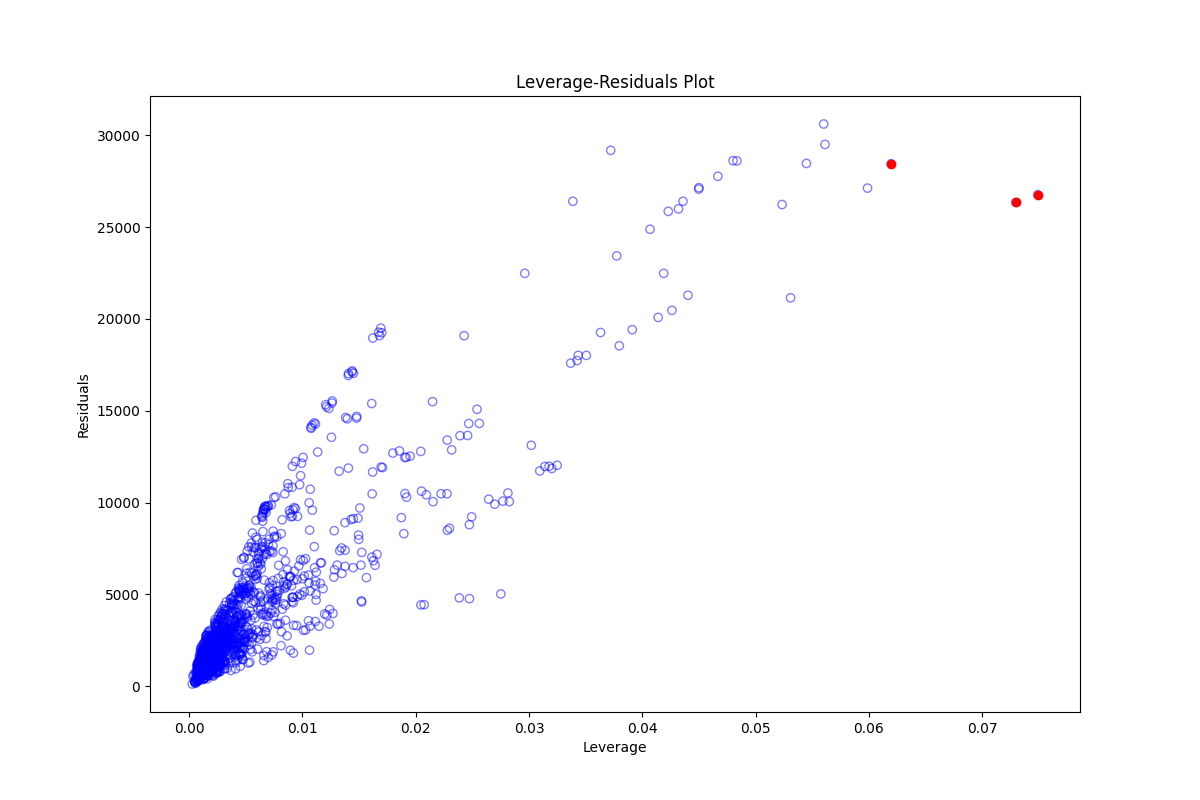
\includegraphics[width=0.9\linewidth]{images/FeOT_Full_4.png}
    \caption{Iteration 4 (RMSE = 1.90)}
    \label{fig:iteration4}
\end{subfigure}

% Third Row
% \begin{subfigure}{\textwidth}
%     \centering
%     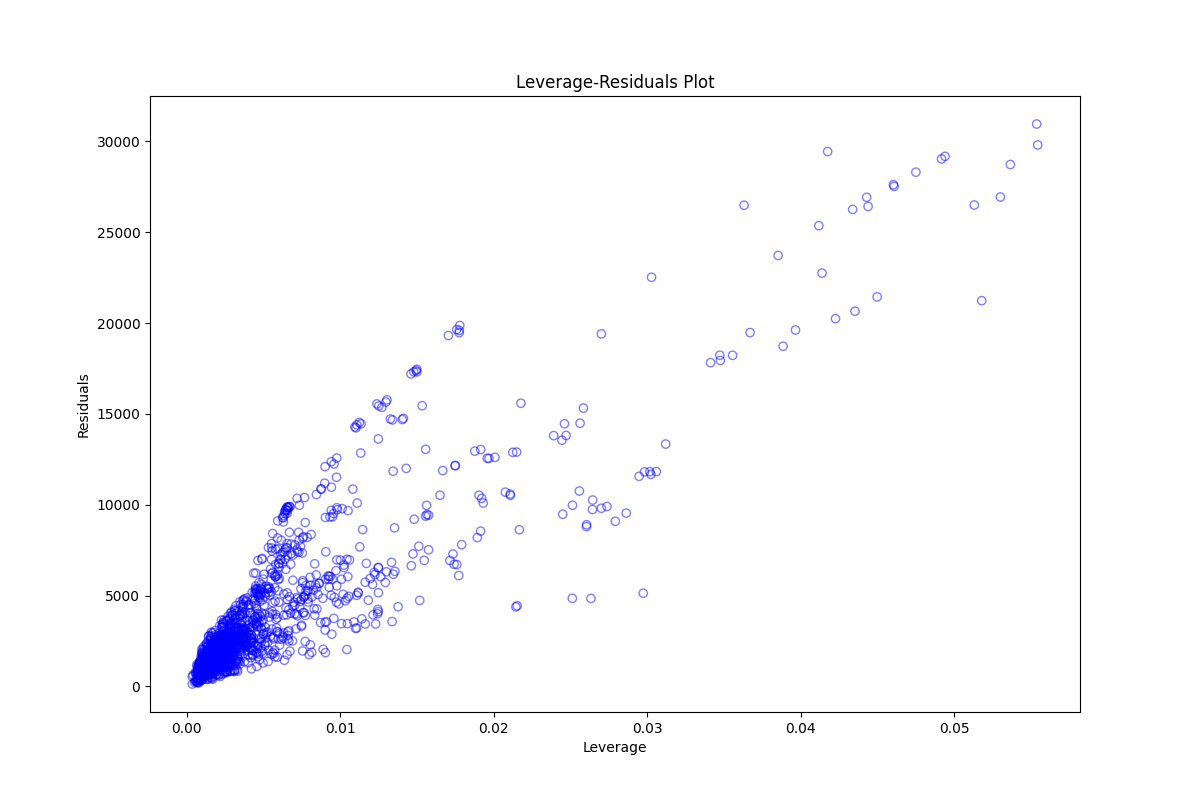
\includegraphics[width=0.45\textwidth]{images/FeOT_Full_5.png}
%     \caption{Iteration 5}
%     \label{fig:iteration5}
% \end{subfigure}

\caption{The results of the outlier removal process for the FeOT submodel. The red dots represent the outliers that were removed in each iteration.}
\label{fig:FeOT_oxide_removal}
\end{figure*}


\subsection{ICA}\label{sec:methodology_ica}
The ICA phase in our pipeline can be seen in figure \ref{fig:ica_phase}.
In this section, we delve into the differences between our pipeline and the original, and we discuss the rationale behind our choices.

\begin{figure}
	\centering
	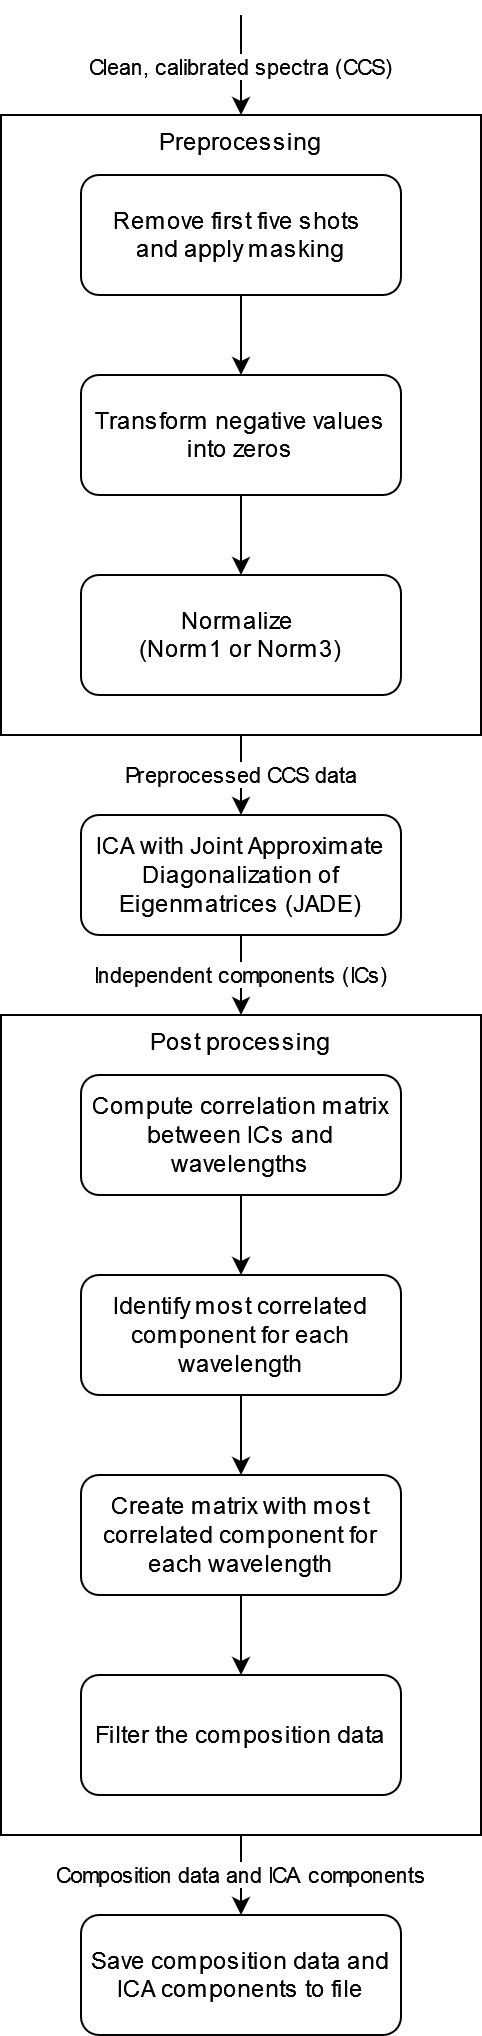
\includegraphics[width=0.2675\textwidth]{images/ica_phase.png}
	\caption{The ICA phase in our recreation of the pipeline.}
	\label{fig:ica_phase}
\end{figure}

\subsubsection{Data Preprocessing}\label{sec:ica_data_preprocessing}
For ICA, the first five shots are removed from the data.
We then apply masking to the data by zeroing out the same regions as in the PLS1-SM phase.
Afterwards, we transform all negative values into zeros.
Then we normalize the data using Norm1 and Norm3.

In contrast to \citet{cleggRecalibrationMarsScience2017} however, we do not weigh by the inverse of the instrument response function (IRF) before normalizing.
The purpose of the IRF is to calibrate the measured signal to physical units since different pixels have different sensitivities\cite{wiensChemcam2012}.
One argument for inverting the IRF is that it introduces more noise in areas of interest on the spectrum by multiplying with a high value as part of the conversion to physical units.
However, during a conversation with one of the original authors of \citet{cleggRecalibrationMarsScience2017}, criticism was raised against this.
Specifically, the author pointed out that weighing by the inverse of the discards the alignment between the spectral data collected by the instrument in Los Alamos and the spectral data collected by the instrument on Mars.
If the same instrument were used for all analyses, one could argue that the IRF (apart from the inverse square law correction) part is irrelevant, but that is not the case here; there are two different instruments --- one in Los Alamos and one on Mars.
Based on these considerations, we have decided to not weigh by the inverse of the IRF.

In addition, because \citet{cleggRecalibrationMarsScience2017} does not specify how each of the five location datasets are used for each sample, we have decided to only use one for each sample.
This likely does not produce as accurate results as using all five location datasets would, since we do not get a full representation of the sample that was shot at by the laser, instead only getting a partial representation from a single location.
Nevertheless, to avoid deviating significantly from \citet{cleggRecalibrationMarsScience2017}'s methodology or making unfounded assumptions about their data processing, we have opted for this more conservative approach.
Our goal is to test each of the components of the pipeline individually rather than trying to reproduce the results to absolute perfection.

Similarly, in our replica of the pipeline, we have not incorporated outlier detection in the ICA part of the pipeline primarily because \citet{cleggRecalibrationMarsScience2017} does not describe their implementation sufficiently enough for replication without unsubstantiated assumptions.
They mention the use of Median Absolute Deviation for this purpose, but the specifics of their approach remain unclear.
Our decision to omit outlier detection in the ICA phase of our pipeline is also influenced by a preference for retaining a more comprehensive dataset, despite the potential inclusion of outliers.
Further supporting this decision is input from one of the original authors involved in the ChemCam project.
This author highlighted the extensive efforts invested in developing the ChemCam calibration dataset, suggesting a low presence of significant outliers.
While it would be ideal to include outlier detection in the ICA phase to ensure alignment with the original pipeline, implementing it based on substantial assumptions would be counterproductive, potentially compromising the integrity of our analysis.

After examining the results in section \ref{sec:results}, we will discuss the implications of these design choices in section \ref{sec:discussion}.

\subsubsection{Joint Approximate Diagonalization of Eigenmatrices (JADE) and Regression}
After preprocessing the data, we are ready to perform ICA.
This is done using the Joint Approximate Diagonalization of Eigenmatrices (JADE) algorithm, which is used to calculate the mixing matrix.
This mixing matrix is an $N \times M$ matrix, where $N$ is the number of samples and $M$ is the number of independent components.
By taking the product of the mixing matrix and the normalized data, we get the estimated sources.
This new matrix is an $M \times P$ matrix, where $M$ is the number of independent components, and $P$ is the number of wavelengths.
Our replica of the pipeline uses $M = 8$ independent components, which is the same as \citet{cleggRecalibrationMarsScience2017}.

After performing ICA, we post-process by computing the correlation between the independent components and the wavelengths.
Using this, we can identify which wavelengths are associated with which independent components by computing the maximum correlation for each wavelength.
This gives us a matrix of ICA scores that we then use for regression.

\begin{figure}
	\centering
	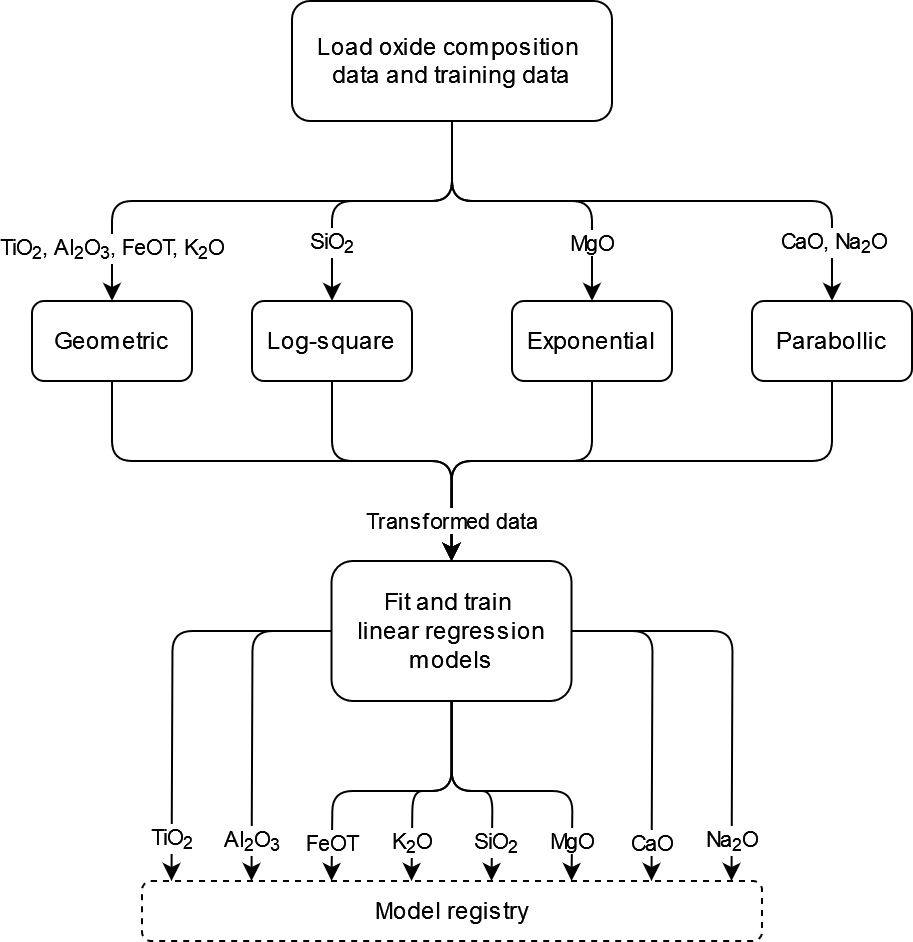
\includegraphics[width=0.45\textwidth]{images/ica_regression.png}
	\caption{Regression in the ICA phase of our recreation of the pipeline.}
	\label{fig:ica_regression}
\end{figure}

The regression process is illustrated in figure \ref{fig:ica_regression}.
\citet{cleggRecalibrationMarsScience2017} perform four more types of regression in addition to linear regression, namely parabolic, exponential, geometric and logsquare.
For each oxide, they used the type of regression and normalization that produced the best results.

We use Linear Regression for all oxides and instead transform the data to fit the model similar to \citet{kuo_detecting_2018}.
Initially, it might appear limiting, but by applying transformations to the features --— for example by taking logs, square roots, etc. --- it's possible to achieve an almost linear relationship with the target variable.

\subsection{MOC}\label{sec:methodology_moc}
As described in section \ref{sec:moc_derivation}, the result of the PLS1-SM and ICA are combined to produce the final MOC model, which weights the results of the two techniques in favor of the one that performs best for each oxide.
The specific weights used for each oxide can be seen in table \ref{tab:weighted_sum_oxide}.

\begin{table}[h]
\centering
\begin{tabular*}{\columnwidth}{@{\extracolsep{\fill}}lll}
\toprule
Element  & PLS1-SM (\%) & ICA (\%) \\ \midrule
Al       & 75           & 25      \\
Fe       & 75           & 25      \\
Si       & 50           & 50      \\
Na       & 40           & 60      \\
K2       & 25           & 75      \\
Ti       & 50           & 50      \\
Mg       & 50           & 50      \\
Ca       & 50           & 50      \\
\bottomrule
\end{tabular*}
\caption{Weighted Sum of Oxide Percentages.}
\label{tab:weighted_sum_oxide}
\end{table}